\documentclass[../../../../doc.tex]{subfiles}

\usepackage[utf8]{inputenc}
\usepackage{polski}

\begin{document}
\subsection{Algorytm DFS}


\subsubsection{Opis działania algorytmu}

Algorytm wykorzystuje \textbf{przeszukiwanie w głąb (Depth-First Search)} do znalezienia ścieżki między punktem startowym a końcowym w labiryncie. Poniżej przedstawiono kluczowe kroki działania.

\subsubsection{Inicjalizacja}
\begin{enumerate}
  \item Inicjalizacja struktur danych:
        \begin{itemize}
          \item \texttt{stack} - stos przechowujący węzły do odwiedzenia (zainicjowany pozycją startową),
          \item \texttt{state} - mapa śledząca stan węzłów (czy węzeł został odwiedzony).
        \end{itemize}
  \item Oznaczenie węzła startowego jako \texttt{queued} (w kolejce).
\end{enumerate}

\subsubsection{Funkcja rekurencyjna DFS}
Główna logika zaimplementowana jest w funkcji rekurencyjnej \texttt{dfs(currentNodePos)} przedstawia algorytm \ref{find_dfs}.

\begin{algorithm}
  \caption{Procedura DFS}
  \label{find_dfs}
  \begin{algorithmic}
    \STATE Oznacz bieżący węzeł jako \texttt{candidate} (kandydat)
    \IF{bieżący węzeł jest metą (\texttt{finish})}
    \STATE Oznacz węzeł jako \texttt{selected} (wybrany)
    \RETURN ścieżka zawierająca tylko bieżący węzeł
    \ENDIF
    \FOR{każdego sąsiada (neighbour) bieżącego węzła}
    \IF{sąsiad nie jest kolizją i nie był odwiedzony (\texttt{candidate/forsaken})}
    \STATE Oznacz sąsiada jako \texttt{queued}
    \STATE $\text{path} \leftarrow \textbf{dfs}\text{(pozycja sasiada)}$
    \IF{ścieżka nie jest pusta}
    \STATE Oznacz bieżący węzeł jako \texttt{selected}
    \STATE Dodaj bieżący węzeł do ścieżki
    \RETURN ścieżka
    \ELSE
    \STATE Oznacz sąsiada jako \texttt{forsaken} (porzucony)
    \ENDIF
    \ENDIF
    \ENDFOR
    \RETURN pusta ścieżka
  \end{algorithmic}
\end{algorithm}

\vspace{-16pt}

\subsubsection{Proces budowania ścieżki}
\begin{enumerate}
  \item \textbf{Propagacja w górę:} Po znalezieniu mety:
        \begin{itemize}
          \item Następuje rekurencyjna propagacja w górę drzewa.
          \item Każdy węzeł dodaje swoją pozycję do ścieżki.
          \item Węzły na ścieżce oznaczane są jako \texttt{selected}.
        \end{itemize}
  \item \textbf{Weryfikacja ścieżki:} Jeśli ścieżka nie istnieje, zwracana jest pusta lista.
  \item \textbf{Końcowe przetwarzanie:} Po zakończeniu rekurencji ścieżka jest odwracana gdyż budowana jest od mety do startu, a wynik powinien przedstawiać kolejność od startu do mety.
\end{enumerate}

\subsubsection{Możliwe stany węzłów}
\begin{itemize}
  \item \texttt{queued} - w kolejce do odwiedzenia,
  \item \texttt{candidate} - aktualnie przetwarzany,
  \item \texttt{selected} - część finalnej ścieżki,
  \item \texttt{forsaken} - porzucony (nie prowadzi do mety).
\end{itemize}

\subsubsection{Złożoność obliczeniowa}
\begin{itemize}
  \item \textbf{Czasowa}: $O(V + E)$, gdzie:
        \begin{itemize}
          \item $V$ - liczba węzłów,
          \item $E$ - liczba krawędzi.
        \end{itemize}
  \item \textbf{Pamięciowa}: $O(V)$, zdeterminowana głębokością rekurencji
\end{itemize}

\noindent Przykład działania algorytmu przedstawiają rysunki \ref{fig:dfs_solve_steps_start}-\ref{fig:dfs_solve_steps_end}.

\vspace{4pt}
\noindent \textit{W opisach rysunków współrzędne \( (x, y) \) oznaczają: \( x \) – kolumna, \( y \) – wiersz, licząc od zera.}

% \begin{multicols}{2}
  
\begin{figure}[H]

  \centering

  \begin{tikzpicture}
    \fill[gray] (1, 0) rectangle (2, 1);
    \fill[gray] (2, 0) rectangle (3, 1);
    \fill[gray] (3, 0) rectangle (4, 1);
    \fill[gray] (2, 1) rectangle (3, 2);
    \fill[gray] (0, 2) rectangle (1, 3);
    \node at (3.5, 2.5){\color{blue}\faIcon{home}};
    \fill[gray] (4, 2) rectangle (5, 3);
    \node at (1.5, 3.5){\color{blue}\faIcon{user}};
    \fill[gray] (2, 3) rectangle (3, 4);
    \fill[gray] (0, 4) rectangle (1, 5);
    \fill[gray] (4, 4) rectangle (5, 5);
    \draw[black] grid (5, 5);
  \end{tikzpicture}

  \caption{Wybierz {"x":1,"y":3} jako następnie rozpatywany węzeł}
  \label{fig:dfs_solve_steps}
\end{figure}

\begin{figure}[H]
  \ContinuedFloat
  \centering

  \begin{tikzpicture}
    \fill[gray] (1, 0) rectangle (2, 1);
    \fill[gray] (2, 0) rectangle (3, 1);
    \fill[gray] (3, 0) rectangle (4, 1);
    \fill[gray] (2, 1) rectangle (3, 2);
    \fill[gray] (0, 2) rectangle (1, 3);
    \node at (3.5, 2.5){\color{blue}\faIcon{home}};
    \fill[gray] (4, 2) rectangle (5, 3);
    \node at (1.5, 3.5){\color{blue}\faIcon{user}};
    \fill[gray] (2, 3) rectangle (3, 4);
    \fill[gray] (0, 4) rectangle (1, 5);
    \fill[gray] (4, 4) rectangle (5, 5);
    \draw[black] grid (5, 5);
  \end{tikzpicture}

  \caption{Oznacz {"x":1,"y":3} jako kandydata}

\end{figure}

\begin{figure}[H]
  \ContinuedFloat
  \centering

  \begin{tikzpicture}
    \fill[gray] (1, 0) rectangle (2, 1);
    \fill[gray] (2, 0) rectangle (3, 1);
    \fill[gray] (3, 0) rectangle (4, 1);
    \fill[gray] (2, 1) rectangle (3, 2);
    \fill[gray] (0, 2) rectangle (1, 3);
    \node at (1.5, 2.5){\color{purple}\faIcon{hourglass}};
    \node at (3.5, 2.5){\color{blue}\faIcon{home}};
    \fill[gray] (4, 2) rectangle (5, 3);
    \node at (1.5, 3.5){\color{blue}\faIcon{user}};
    \fill[gray] (2, 3) rectangle (3, 4);
    \fill[gray] (0, 4) rectangle (1, 5);
    \fill[gray] (4, 4) rectangle (5, 5);
    \draw[black] grid (5, 5);
  \end{tikzpicture}

  \caption{Wybierz {"x":1,"y":2} jako następnie rozpatywany węzeł}

\end{figure}

\begin{figure}[H]
  \ContinuedFloat
  \centering

  \begin{tikzpicture}
    \fill[gray] (1, 0) rectangle (2, 1);
    \fill[gray] (2, 0) rectangle (3, 1);
    \fill[gray] (3, 0) rectangle (4, 1);
    \fill[gray] (2, 1) rectangle (3, 2);
    \fill[gray] (0, 2) rectangle (1, 3);
    \node at (1.5, 2.5){\color{orange}\faIcon{arrows-alt}};
    \node at (3.5, 2.5){\color{blue}\faIcon{home}};
    \fill[gray] (4, 2) rectangle (5, 3);
    \node at (1.5, 3.5){\color{blue}\faIcon{user}};
    \fill[gray] (2, 3) rectangle (3, 4);
    \fill[gray] (0, 4) rectangle (1, 5);
    \fill[gray] (4, 4) rectangle (5, 5);
    \draw[black] grid (5, 5);
  \end{tikzpicture}

  \caption{Oznacz {"x":1,"y":2} jako kandydata}

\end{figure}

\begin{figure}[H]
  \ContinuedFloat
  \centering

  \begin{tikzpicture}
    \fill[gray] (1, 0) rectangle (2, 1);
    \fill[gray] (2, 0) rectangle (3, 1);
    \fill[gray] (3, 0) rectangle (4, 1);
    \node at (1.5, 1.5){\color{purple}\faIcon{hourglass}};
    \fill[gray] (2, 1) rectangle (3, 2);
    \fill[gray] (0, 2) rectangle (1, 3);
    \node at (1.5, 2.5){\color{orange}\faIcon{arrows-alt}};
    \node at (3.5, 2.5){\color{blue}\faIcon{home}};
    \fill[gray] (4, 2) rectangle (5, 3);
    \node at (1.5, 3.5){\color{blue}\faIcon{user}};
    \fill[gray] (2, 3) rectangle (3, 4);
    \fill[gray] (0, 4) rectangle (1, 5);
    \fill[gray] (4, 4) rectangle (5, 5);
    \draw[black] grid (5, 5);
  \end{tikzpicture}

  \caption{Wybierz {"x":1,"y":1} jako następnie rozpatywany węzeł}

\end{figure}

\begin{figure}[H]
  \ContinuedFloat
  \centering

  \begin{tikzpicture}
    \fill[gray] (1, 0) rectangle (2, 1);
    \fill[gray] (2, 0) rectangle (3, 1);
    \fill[gray] (3, 0) rectangle (4, 1);
    \node at (1.5, 1.5){\color{orange}\faIcon{arrows-alt}};
    \fill[gray] (2, 1) rectangle (3, 2);
    \fill[gray] (0, 2) rectangle (1, 3);
    \node at (1.5, 2.5){\color{orange}\faIcon{arrows-alt}};
    \node at (3.5, 2.5){\color{blue}\faIcon{home}};
    \fill[gray] (4, 2) rectangle (5, 3);
    \node at (1.5, 3.5){\color{blue}\faIcon{user}};
    \fill[gray] (2, 3) rectangle (3, 4);
    \fill[gray] (0, 4) rectangle (1, 5);
    \fill[gray] (4, 4) rectangle (5, 5);
    \draw[black] grid (5, 5);
  \end{tikzpicture}

  \caption{Oznacz {"x":1,"y":1} jako kandydata}

\end{figure}

\begin{figure}[H]
  \ContinuedFloat
  \centering

  \begin{tikzpicture}
    \fill[gray] (1, 0) rectangle (2, 1);
    \fill[gray] (2, 0) rectangle (3, 1);
    \fill[gray] (3, 0) rectangle (4, 1);
    \node at (0.5, 1.5){\color{purple}\faIcon{hourglass}};
    \node at (1.5, 1.5){\color{orange}\faIcon{arrows-alt}};
    \fill[gray] (2, 1) rectangle (3, 2);
    \fill[gray] (0, 2) rectangle (1, 3);
    \node at (1.5, 2.5){\color{orange}\faIcon{arrows-alt}};
    \node at (3.5, 2.5){\color{blue}\faIcon{home}};
    \fill[gray] (4, 2) rectangle (5, 3);
    \node at (1.5, 3.5){\color{blue}\faIcon{user}};
    \fill[gray] (2, 3) rectangle (3, 4);
    \fill[gray] (0, 4) rectangle (1, 5);
    \fill[gray] (4, 4) rectangle (5, 5);
    \draw[black] grid (5, 5);
  \end{tikzpicture}

  \caption{Wybierz {"x":0,"y":1} jako następnie rozpatywany węzeł}

\end{figure}

\begin{figure}[H]
  \ContinuedFloat
  \centering

  \begin{tikzpicture}
    \fill[gray] (1, 0) rectangle (2, 1);
    \fill[gray] (2, 0) rectangle (3, 1);
    \fill[gray] (3, 0) rectangle (4, 1);
    \node at (0.5, 1.5){\color{orange}\faIcon{arrows-alt}};
    \node at (1.5, 1.5){\color{orange}\faIcon{arrows-alt}};
    \fill[gray] (2, 1) rectangle (3, 2);
    \fill[gray] (0, 2) rectangle (1, 3);
    \node at (1.5, 2.5){\color{orange}\faIcon{arrows-alt}};
    \node at (3.5, 2.5){\color{blue}\faIcon{home}};
    \fill[gray] (4, 2) rectangle (5, 3);
    \node at (1.5, 3.5){\color{blue}\faIcon{user}};
    \fill[gray] (2, 3) rectangle (3, 4);
    \fill[gray] (0, 4) rectangle (1, 5);
    \fill[gray] (4, 4) rectangle (5, 5);
    \draw[black] grid (5, 5);
  \end{tikzpicture}

  \caption{Oznacz {"x":0,"y":1} jako kandydata}

\end{figure}

\begin{figure}[H]
  \ContinuedFloat
  \centering

  \begin{tikzpicture}
    \node at (0.5, 0.5){\color{purple}\faIcon{hourglass}};
    \fill[gray] (1, 0) rectangle (2, 1);
    \fill[gray] (2, 0) rectangle (3, 1);
    \fill[gray] (3, 0) rectangle (4, 1);
    \node at (0.5, 1.5){\color{orange}\faIcon{arrows-alt}};
    \node at (1.5, 1.5){\color{orange}\faIcon{arrows-alt}};
    \fill[gray] (2, 1) rectangle (3, 2);
    \fill[gray] (0, 2) rectangle (1, 3);
    \node at (1.5, 2.5){\color{orange}\faIcon{arrows-alt}};
    \node at (3.5, 2.5){\color{blue}\faIcon{home}};
    \fill[gray] (4, 2) rectangle (5, 3);
    \node at (1.5, 3.5){\color{blue}\faIcon{user}};
    \fill[gray] (2, 3) rectangle (3, 4);
    \fill[gray] (0, 4) rectangle (1, 5);
    \fill[gray] (4, 4) rectangle (5, 5);
    \draw[black] grid (5, 5);
  \end{tikzpicture}

  \caption{Wybierz {"x":0,"y":0} jako następnie rozpatywany węzeł}

\end{figure}

\begin{figure}[H]
  \ContinuedFloat
  \centering

  \begin{tikzpicture}
    \node at (0.5, 0.5){\color{orange}\faIcon{arrows-alt}};
    \fill[gray] (1, 0) rectangle (2, 1);
    \fill[gray] (2, 0) rectangle (3, 1);
    \fill[gray] (3, 0) rectangle (4, 1);
    \node at (0.5, 1.5){\color{orange}\faIcon{arrows-alt}};
    \node at (1.5, 1.5){\color{orange}\faIcon{arrows-alt}};
    \fill[gray] (2, 1) rectangle (3, 2);
    \fill[gray] (0, 2) rectangle (1, 3);
    \node at (1.5, 2.5){\color{orange}\faIcon{arrows-alt}};
    \node at (3.5, 2.5){\color{blue}\faIcon{home}};
    \fill[gray] (4, 2) rectangle (5, 3);
    \node at (1.5, 3.5){\color{blue}\faIcon{user}};
    \fill[gray] (2, 3) rectangle (3, 4);
    \fill[gray] (0, 4) rectangle (1, 5);
    \fill[gray] (4, 4) rectangle (5, 5);
    \draw[black] grid (5, 5);
  \end{tikzpicture}

  \caption{Oznacz {"x":0,"y":0} jako kandydata}

\end{figure}

\begin{figure}[H]
  \ContinuedFloat
  \centering

  \begin{tikzpicture}
    \node at (0.5, 0.5){\color{orange}\faIcon{arrows-alt}};
    \fill[gray] (1, 0) rectangle (2, 1);
    \fill[gray] (2, 0) rectangle (3, 1);
    \fill[gray] (3, 0) rectangle (4, 1);
    \node at (0.5, 1.5){\color{orange}\faIcon{arrows-alt}};
    \node at (1.5, 1.5){\color{orange}\faIcon{arrows-alt}};
    \fill[gray] (2, 1) rectangle (3, 2);
    \fill[gray] (0, 2) rectangle (1, 3);
    \node at (1.5, 2.5){\color{orange}\faIcon{arrows-alt}};
    \node at (3.5, 2.5){\color{blue}\faIcon{home}};
    \fill[gray] (4, 2) rectangle (5, 3);
    \node at (1.5, 3.5){\color{blue}\faIcon{user}};
    \fill[gray] (2, 3) rectangle (3, 4);
    \fill[gray] (0, 4) rectangle (1, 5);
    \fill[gray] (4, 4) rectangle (5, 5);
    \draw[black] grid (5, 5);
  \end{tikzpicture}

  \caption{Oznacz {"x":0,"y":0} jako zapomniany}

\end{figure}

\begin{figure}[H]
  \ContinuedFloat
  \centering

  \begin{tikzpicture}
    \node at (0.5, 0.5){\color{red}\faIcon{skull}};
    \fill[gray] (1, 0) rectangle (2, 1);
    \fill[gray] (2, 0) rectangle (3, 1);
    \fill[gray] (3, 0) rectangle (4, 1);
    \node at (0.5, 1.5){\color{orange}\faIcon{arrows-alt}};
    \node at (1.5, 1.5){\color{orange}\faIcon{arrows-alt}};
    \fill[gray] (2, 1) rectangle (3, 2);
    \fill[gray] (0, 2) rectangle (1, 3);
    \node at (1.5, 2.5){\color{orange}\faIcon{arrows-alt}};
    \node at (3.5, 2.5){\color{blue}\faIcon{home}};
    \fill[gray] (4, 2) rectangle (5, 3);
    \node at (1.5, 3.5){\color{blue}\faIcon{user}};
    \fill[gray] (2, 3) rectangle (3, 4);
    \fill[gray] (0, 4) rectangle (1, 5);
    \fill[gray] (4, 4) rectangle (5, 5);
    \draw[black] grid (5, 5);
  \end{tikzpicture}

  \caption{Oznacz {"x":0,"y":1} jako zapomniany}

\end{figure}

\begin{figure}[H]
  \ContinuedFloat
  \centering

  \begin{tikzpicture}
    \node at (0.5, 0.5){\color{red}\faIcon{skull}};
    \fill[gray] (1, 0) rectangle (2, 1);
    \fill[gray] (2, 0) rectangle (3, 1);
    \fill[gray] (3, 0) rectangle (4, 1);
    \node at (0.5, 1.5){\color{red}\faIcon{skull}};
    \node at (1.5, 1.5){\color{orange}\faIcon{arrows-alt}};
    \fill[gray] (2, 1) rectangle (3, 2);
    \fill[gray] (0, 2) rectangle (1, 3);
    \node at (1.5, 2.5){\color{orange}\faIcon{arrows-alt}};
    \node at (3.5, 2.5){\color{blue}\faIcon{home}};
    \fill[gray] (4, 2) rectangle (5, 3);
    \node at (1.5, 3.5){\color{blue}\faIcon{user}};
    \fill[gray] (2, 3) rectangle (3, 4);
    \fill[gray] (0, 4) rectangle (1, 5);
    \fill[gray] (4, 4) rectangle (5, 5);
    \draw[black] grid (5, 5);
  \end{tikzpicture}

  \caption{Oznacz {"x":1,"y":1} jako zapomniany}

\end{figure}

\begin{figure}[H]
  \ContinuedFloat
  \centering

  \begin{tikzpicture}
    \node at (0.5, 0.5){\color{red}\faIcon{skull}};
    \fill[gray] (1, 0) rectangle (2, 1);
    \fill[gray] (2, 0) rectangle (3, 1);
    \fill[gray] (3, 0) rectangle (4, 1);
    \node at (0.5, 1.5){\color{red}\faIcon{skull}};
    \node at (1.5, 1.5){\color{red}\faIcon{skull}};
    \fill[gray] (2, 1) rectangle (3, 2);
    \fill[gray] (0, 2) rectangle (1, 3);
    \node at (1.5, 2.5){\color{orange}\faIcon{arrows-alt}};
    \node at (2.5, 2.5){\color{purple}\faIcon{hourglass}};
    \node at (3.5, 2.5){\color{blue}\faIcon{home}};
    \fill[gray] (4, 2) rectangle (5, 3);
    \node at (1.5, 3.5){\color{blue}\faIcon{user}};
    \fill[gray] (2, 3) rectangle (3, 4);
    \fill[gray] (0, 4) rectangle (1, 5);
    \fill[gray] (4, 4) rectangle (5, 5);
    \draw[black] grid (5, 5);
  \end{tikzpicture}

  \caption{Wybierz {"x":2,"y":2} jako następnie rozpatywany węzeł}

\end{figure}

\begin{figure}[H]
  \ContinuedFloat
  \centering

  \begin{tikzpicture}
    \node at (0.5, 0.5){\color{red}\faIcon{skull}};
    \fill[gray] (1, 0) rectangle (2, 1);
    \fill[gray] (2, 0) rectangle (3, 1);
    \fill[gray] (3, 0) rectangle (4, 1);
    \node at (0.5, 1.5){\color{red}\faIcon{skull}};
    \node at (1.5, 1.5){\color{red}\faIcon{skull}};
    \fill[gray] (2, 1) rectangle (3, 2);
    \fill[gray] (0, 2) rectangle (1, 3);
    \node at (1.5, 2.5){\color{orange}\faIcon{arrows-alt}};
    \node at (2.5, 2.5){\color{orange}\faIcon{arrows-alt}};
    \node at (3.5, 2.5){\color{blue}\faIcon{home}};
    \fill[gray] (4, 2) rectangle (5, 3);
    \node at (1.5, 3.5){\color{blue}\faIcon{user}};
    \fill[gray] (2, 3) rectangle (3, 4);
    \fill[gray] (0, 4) rectangle (1, 5);
    \fill[gray] (4, 4) rectangle (5, 5);
    \draw[black] grid (5, 5);
  \end{tikzpicture}

  \caption{Oznacz {"x":2,"y":2} jako kandydata}

\end{figure}

\begin{figure}[H]
  \ContinuedFloat
  \centering

  \begin{tikzpicture}
    \node at (0.5, 0.5){\color{red}\faIcon{skull}};
    \fill[gray] (1, 0) rectangle (2, 1);
    \fill[gray] (2, 0) rectangle (3, 1);
    \fill[gray] (3, 0) rectangle (4, 1);
    \node at (0.5, 1.5){\color{red}\faIcon{skull}};
    \node at (1.5, 1.5){\color{red}\faIcon{skull}};
    \fill[gray] (2, 1) rectangle (3, 2);
    \fill[gray] (0, 2) rectangle (1, 3);
    \node at (1.5, 2.5){\color{orange}\faIcon{arrows-alt}};
    \node at (2.5, 2.5){\color{orange}\faIcon{arrows-alt}};
    \node at (3.5, 2.5){\color{blue}\faIcon{home}};
    \fill[gray] (4, 2) rectangle (5, 3);
    \node at (1.5, 3.5){\color{blue}\faIcon{user}};
    \fill[gray] (2, 3) rectangle (3, 4);
    \fill[gray] (0, 4) rectangle (1, 5);
    \fill[gray] (4, 4) rectangle (5, 5);
    \draw[black] grid (5, 5);
  \end{tikzpicture}

  \caption{Wybierz {"x":3,"y":2} jako następnie rozpatywany węzeł}

\end{figure}

\begin{figure}[H]
  \ContinuedFloat
  \centering

  \begin{tikzpicture}
    \node at (0.5, 0.5){\color{red}\faIcon{skull}};
    \fill[gray] (1, 0) rectangle (2, 1);
    \fill[gray] (2, 0) rectangle (3, 1);
    \fill[gray] (3, 0) rectangle (4, 1);
    \node at (0.5, 1.5){\color{red}\faIcon{skull}};
    \node at (1.5, 1.5){\color{red}\faIcon{skull}};
    \fill[gray] (2, 1) rectangle (3, 2);
    \fill[gray] (0, 2) rectangle (1, 3);
    \node at (1.5, 2.5){\color{orange}\faIcon{arrows-alt}};
    \node at (2.5, 2.5){\color{orange}\faIcon{arrows-alt}};
    \node at (3.5, 2.5){\color{blue}\faIcon{home}};
    \fill[gray] (4, 2) rectangle (5, 3);
    \node at (1.5, 3.5){\color{blue}\faIcon{user}};
    \fill[gray] (2, 3) rectangle (3, 4);
    \fill[gray] (0, 4) rectangle (1, 5);
    \fill[gray] (4, 4) rectangle (5, 5);
    \draw[black] grid (5, 5);
  \end{tikzpicture}

  \caption{Oznacz {"x":3,"y":2} jako kandydata}

\end{figure}

\begin{figure}[H]
  \ContinuedFloat
  \centering

  \begin{tikzpicture}
    \node at (0.5, 0.5){\color{red}\faIcon{skull}};
    \fill[gray] (1, 0) rectangle (2, 1);
    \fill[gray] (2, 0) rectangle (3, 1);
    \fill[gray] (3, 0) rectangle (4, 1);
    \node at (0.5, 1.5){\color{red}\faIcon{skull}};
    \node at (1.5, 1.5){\color{red}\faIcon{skull}};
    \fill[gray] (2, 1) rectangle (3, 2);
    \fill[gray] (0, 2) rectangle (1, 3);
    \node at (1.5, 2.5){\color{orange}\faIcon{arrows-alt}};
    \node at (2.5, 2.5){\color{orange}\faIcon{arrows-alt}};
    \node at (3.5, 2.5){\color{blue}\faIcon{home}};
    \fill[gray] (4, 2) rectangle (5, 3);
    \node at (1.5, 3.5){\color{blue}\faIcon{user}};
    \fill[gray] (2, 3) rectangle (3, 4);
    \fill[gray] (0, 4) rectangle (1, 5);
    \fill[gray] (4, 4) rectangle (5, 5);
    \draw[black] grid (5, 5);
  \end{tikzpicture}

  \caption{Wybierz {"x":3,"y":2} do finalnej ścierzki}

\end{figure}

\begin{figure}[H]
  \ContinuedFloat
  \centering

  \begin{tikzpicture}
    \node at (0.5, 0.5){\color{red}\faIcon{skull}};
    \fill[gray] (1, 0) rectangle (2, 1);
    \fill[gray] (2, 0) rectangle (3, 1);
    \fill[gray] (3, 0) rectangle (4, 1);
    \node at (0.5, 1.5){\color{red}\faIcon{skull}};
    \node at (1.5, 1.5){\color{red}\faIcon{skull}};
    \fill[gray] (2, 1) rectangle (3, 2);
    \fill[gray] (0, 2) rectangle (1, 3);
    \node at (1.5, 2.5){\color{orange}\faIcon{arrows-alt}};
    \node at (2.5, 2.5){\color{green}\faIcon{check}};
    \node at (3.5, 2.5){\color{blue}\faIcon{home}};
    \fill[gray] (4, 2) rectangle (5, 3);
    \node at (1.5, 3.5){\color{blue}\faIcon{user}};
    \fill[gray] (2, 3) rectangle (3, 4);
    \fill[gray] (0, 4) rectangle (1, 5);
    \fill[gray] (4, 4) rectangle (5, 5);
    \draw[black] grid (5, 5);
  \end{tikzpicture}

  \caption{Wybierz {"x":2,"y":2} do finalnej ścierzki}

\end{figure}

\begin{figure}[H]
  \ContinuedFloat
  \centering

  \begin{tikzpicture}
    \node at (0.5, 0.5){\color{red}\faIcon{skull}};
    \fill[gray] (1, 0) rectangle (2, 1);
    \fill[gray] (2, 0) rectangle (3, 1);
    \fill[gray] (3, 0) rectangle (4, 1);
    \node at (0.5, 1.5){\color{red}\faIcon{skull}};
    \node at (1.5, 1.5){\color{red}\faIcon{skull}};
    \fill[gray] (2, 1) rectangle (3, 2);
    \fill[gray] (0, 2) rectangle (1, 3);
    \node at (1.5, 2.5){\color{green}\faIcon{check}};
    \node at (2.5, 2.5){\color{green}\faIcon{check}};
    \node at (3.5, 2.5){\color{blue}\faIcon{home}};
    \fill[gray] (4, 2) rectangle (5, 3);
    \node at (1.5, 3.5){\color{blue}\faIcon{user}};
    \fill[gray] (2, 3) rectangle (3, 4);
    \fill[gray] (0, 4) rectangle (1, 5);
    \fill[gray] (4, 4) rectangle (5, 5);
    \draw[black] grid (5, 5);
  \end{tikzpicture}

  \caption{Wybierz {"x":1,"y":2} do finalnej ścierzki}

\end{figure}

\begin{figure}[H]
  \ContinuedFloat
  \centering

  \begin{tikzpicture}
    \node at (0.5, 0.5){\color{red}\faIcon{skull}};
    \fill[gray] (1, 0) rectangle (2, 1);
    \fill[gray] (2, 0) rectangle (3, 1);
    \fill[gray] (3, 0) rectangle (4, 1);
    \node at (0.5, 1.5){\color{red}\faIcon{skull}};
    \node at (1.5, 1.5){\color{red}\faIcon{skull}};
    \fill[gray] (2, 1) rectangle (3, 2);
    \fill[gray] (0, 2) rectangle (1, 3);
    \node at (1.5, 2.5){\color{green}\faIcon{check}};
    \node at (2.5, 2.5){\color{green}\faIcon{check}};
    \node at (3.5, 2.5){\color{blue}\faIcon{home}};
    \fill[gray] (4, 2) rectangle (5, 3);
    \node at (1.5, 3.5){\color{blue}\faIcon{user}};
    \fill[gray] (2, 3) rectangle (3, 4);
    \fill[gray] (0, 4) rectangle (1, 5);
    \fill[gray] (4, 4) rectangle (5, 5);
    \draw[black] grid (5, 5);
  \end{tikzpicture}

  \caption{Wybierz {"x":1,"y":3} do finalnej ścierzki}

\end{figure}

% \end{multicols}

\end{document}